\documentclass{article}
\usepackage{tikz, comment}
\usepackage{pifont}
\usepackage{fontspec, pgfplots}
\usetikzlibrary{arrows, decorations.markings, decorations.pathreplacing}
\begin{comment}
:Title: Not defined yet
:Tags: moment;apothem;focus of a parabola;perimeter;directrix of a parabola
:Prob: 0.5748;0.5414;0.5342;0.5131;0.5128
:Author: Prof.Hu Ji-shan, HKUST
:Slug: No name yet

Description Here.........
\end{comment}
\begin{document}\centering 

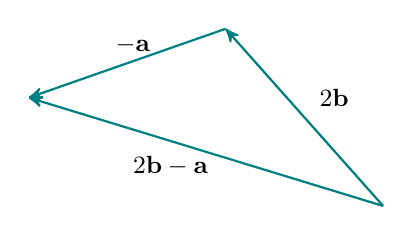
\begin{tikzpicture}[>=latex,xscale=.5*5, yscale=.5*5][font=\sf\small] 

\draw[teal, thick, ->, >=stealth'] (0, 0) -- ({-0.4*2}, {0.45*2})node[black, right, midway, pos=0.5, xshift=2, yshift=7, scale=1]{$2\bf b$}; %2b


\begin{scope}[xshift=-0.8cm,yshift=0.9cm]

\draw[teal, thick, ->, >=stealth'] (0, 0) -- ({1*(-1)}, {0.35*(-1)})node[black, above, midway, pos=0.5, xshift=2, yshift=0, scale=1]{$\bf -a$}; %-a

\end{scope}

\draw[teal, thick, ->, >=stealth'] (0, 0) -- ({-0.8+1*(-1)}, {0.9+0.35*(-1)})node[black, below, midway, pos=0.6, xshift=0, yshift=-2, scale=1]{$2 \bf b - a$}; %2b-a

\end{tikzpicture}
\end{document}